% TODO THOMAS:
% * ACL (inkl. lab)
% * D? Physical hardening
% * D? config as appendix
% * D? delete risk about natural disaster at branch
% * D? flavortext about ict section
% * D? update diagram section
% * D? skim through WAN section
% * D? Generally add stuff about Firewall
% * note about how we did VPN in packet tracer
% * double check wireless security (discussion)
% * add prefix to \refs. "section \ref{..}" for example

%TODO not important:
% * add prefix to \refs. "section \ref{..}" for example
% * fix up ~ before \ref and \cite

% TODO: 
% * ACLs
% * IPsec -> IPSec
% * consistent periods in security policy (and everwhere else for that matter)
% * D? note in WAN section about our demo should be moved to the demo section HVA MENER DU!
% * make sure sections about HQ and branch appear in a consistent order :D *muh consistency*
% * fix up ~ before \ref and \cite
% * D? give lab access switches special treatment?
% * do we want to clearpage before \sections?
% * clean up \\\\'s to look good and uniform
% * Run spellchecker
% * call our PT implementation a demo?
% * branch -> learning centre
% * formatting for IP addresses? :/


% TODO: 
% * ACLs
% ** IPsec -> IPSec (other way around)
% ** consistent periods in security policy (and everwhere else for that matter)
% ** note in WAN section about our demo should be moved to the demo section HVA MENER DU!
% * make sure sections about HQ and branch appear in a consistent order :D *muh consistency*
% * give lab access switches special treatment?
% ** Phyical security!
% ** replace "'S" with "'s"
% * Gjøre guests større? HAKKE TID?
% *                                   Make it clear that we are focusing on saving costs. Redundancy at the HQ for example is a luxury
% ** Setup a pingable host in the services segment to use for demonstration
% ** Write about firewalls, defence-in-depth, etc. in ICT discussion
=======
% * formatting for IP addresses? :/
% * replace "'S" with "'s"
% * D? branch -> learning centre
% * Gjøre guests større?
% * Make it clear that we are focusing on saving costs. Redundancy at the HQ for example is a luxury
% * D? Setup a pingable host in the services segment to use for demonstration
% * D? Write about firewalls, defence-in-depth, etc. in ICT discussion
>>>>>>> origin/sharelatex-2018-11-16-1847

% command to make notes to us in the document
\newcommand{\notetous}[1] {
  \textbf{\textit{\textcolor{red}{#1}}}
}

\documentclass[a4paper,11pt,pdftex,english]{article} % change to norsk for Norwegian abstract and references

\usepackage{babel}
\usepackage{amsmath}
\usepackage{graphicx}
\usepackage[utf8]{inputenc}
\usepackage{epsfig}
\usepackage{graphicx}
\usepackage{palatino}
\renewcommand{\ttdefault}{lmtt}
\usepackage{enumerate}
\usepackage{mdwlist}
\usepackage{geometry}
%\usepackage{textcomp}
%\usepackage{type1cm}
\usepackage[table]{xcolor}
\usepackage{varioref}
\usepackage{url}
\usepackage[bookmarks=true, linkcolor=blue,
citecolor=blue,urlcolor=blue,colorli nks=true, breaklinks=true,
pagebackref=true, hyperindex=true,bookmarksopen=true]{hyperref}
\usepackage[shortlabels]{enumitem}
\newlist{arrowlist}{itemize}{1}
\setlist[arrowlist]{label=$\Rightarrow$}
\usepackage{minted}
\usepackage[strings]{underscore}
\usepackage{dirtytalk}

\graphicspath{ {./images/} } % make LaTeX look for images in the images folder


\frenchspacing

%% Block style paragrphs
\setlength\parskip{\medskipamount}
\setlength\parindent{0pt}

\makeatletter
\renewcommand{\topfraction}{.9}
\renewcommand{\bottomfraction}{.8}
\renewcommand{\textfraction}{.15}
\renewcommand{\floatpagefraction}{.66}
\renewcommand{\dbltopfraction}{.66}
\renewcommand{\dblfloatpagefraction}{.66}
\setcounter{topnumber}{9}
\setcounter{bottomnumber}{9}
\setcounter{totalnumber}{20}
\setcounter{dbltopnumber}{9}

\makeatother



\title{Charity organisation - "SikreNorge"}

% TODO: replace 923 with actual student number
\author{
  Job Nestor Bahner, 494300\\
  Johannes Borgen, 494336\\
  Abdisalan Mohamed Hussein, 494334\\
  Thomas Løkkeborg, 473157\\
}

\begin{document}

\maketitle

\begin{abstract}
SikreNorge is a non-profit charity organisation with locations all over Norway. In this report we discuss how we would implement a network infrastructure for the organisation.
\end{abstract}

\thispagestyle{empty}

\clearpage
\pagenumbering{roman}
\setcounter{page}{1}
\tableofcontents

\clearpage
\pagenumbering{arabic}

% BEGINNING OF CONTENT

\section{Business case}

SikreNorge is a non-profit charity organisation that provides information security services to businesses and institutions in Norway. The organisation seeks to secure Norway by helping those who would not otherwise have the means to prioritize security.

\subsection{Background} % FIXME: new name?

\notetous{Either change section title or add a bit more background :d}

The organisation is reliant on local expertise in each county in the form of volunteers and hired professionals. Volunteers are expected and encouraged to gain security competence through the experts. Good candidates for volunteers are students doing technical studies. Where possible the organisation will make agreements with local universities teaching information technology courses to encourage students to volunteer. The organisation is also open to volunteer work as part of theses and course projects. Volunteers of the organisation do work in exchange for practical information security experience. Both volunteers and hired professionals are expected to sign strict non-disclosure agreements regarding their work with businesses and institutions.
\\
\\
Financially SikreNorge relies on donations, government subsidies, and income from their webshop. Businesses who donate are encouraged to publicise their contribution to show that they support the organisations mission. This way both the contributing businesses and SikreNorge get good PR. Government subsidies are given with the intention and expectation that the organisation will use these means to support local public and private institutions with information security tasks.

\subsection{Locations}

SikreNorge will establish learning centres in each of Norway's 18 counties. The headquarter lies in Oslo. Because of the county merges coming in a couple of years, then we will have to merge our branches.

% TODO note that the number of counties is changing
Learning centres are meant as a hub for all the organisations activities in the county. The centres have offices for local management and hired professionals. They also contain network sandbox areas for practicing network security, classrooms for security courses, lecture halls for seminars and general storage space. In addition to activities held at the centres, the organisation can send consultants into the field to do evaluation or configuration on-site. Consultants are a mix of local hired professionals, volunteers and staff.
\\
\\
The organisations Headquarters, hereafter called HQ, provides the same services as learning centres, but also does the heavy lifting in terms of information technology services and infrastructure. The organisations headquarter provides the same services as learning centres, but also does the heavy lifting in terms of information technology services and infrastructure. The website, E-mail, databases and management applications are examples of services that are hosted here.

\subsection{Services}

The organisation includes a wide range of services, and the network must be set up to support these. Following is a brief discussion of key services, along with some infrastructure concerns.

% TODO more services?

\subsubsection{On-site company consultation}

Volunteers, hired professionals and staff  can be sent out to do consulting on-site at businesses or institutions. Access to the organisations internal services might be required during consultation, so the consultants should be able to reach them from on-site. Confidential information might be sent and received during this communication, so the technology chosen for this should focus on security.

\subsubsection{Teaching at learning centre}

Businesses and institutions may visit a learning centre to take courses or to receive guidance. During this stay they will naturally want internet connectivity. In addition, access to some internal services might be needed for training purposes. A visitors access rights should be restricted as much as possible.

\subsubsection{Network security laboratory}

Each learning centre has a laboratory where visitors can explore hardware and software to learn about vulnerabilities and best practises. Labs are meant to be a sandbox area for learning about information security, so they should be set up with care so that experiments from the lab cannot interfere with the rest of the learning centres operations.

% TODO "separated from the rest of the distribution system" - currently this is not done

\subsubsection{Public website}

SikreNorge's website includes information about the organisations offerings, online courses and a webshop. Some of the website's information and courses might build upon internal services, so the infrastructure should support communication to allow this. The webshop will sell T-shirts, coffee mugs, posters and more to further information security awareness and good practise. The shop allows buyers to register accounts for easy shopping.

\subsubsection{Management website}

The organisation uses a website separate to the public website to manage internal logistics. Registered staff, businesses, institutions and overview of future work are examples of information that can be found here.

% TODO: refer do the bave and below sections in the ict implementation discussion

\section{Security Policy}

% NOTE BY THOMAS: This list was slightly changed from the one in docs, as LaTeX struggles with lists deeper than 4 levels :p

\subsection{Statement of policy}

\begin{enumerate}
  \item Scope and applicability
  \begin{enumerate}
    \item Our organization
      \begin{enumerate}
        \item Every member is expected to know the content of our policy and comply. Ignorance is equal to non compliance.
      \end{enumerate}
        \item Partners
      \begin{enumerate}
        \item They are expected to learn and know the content, whereas an equal understanding of security is key.
      \end{enumerate}
        \item Guests/Trainees
      \begin{enumerate}
        \item Must know key elements to ensure safe learning and usage when using our equipment. Coordinators must brief them before actual usage.
      \end{enumerate}
  \end{enumerate}
\end{enumerate}

\subsection{Responsibilities}

\begin{enumerate}
  \item Chief Executive Officer (CEO)
   \begin{enumerate}
      \item Responsible for the organizations success.
      \item Executives report to the CEO.
  \end{enumerate}
  \item Chief Technology Officer (CTO)
   \begin{enumerate}
      \item Responsible for technology infrastructure
      \begin{enumerate}
        \item Identify and evaluate new technology.
        \item Maintaining and improving existing systems.
        \item Give and delegate counseling about technology to clients.
      \end{enumerate}
  \end{enumerate}
  \item Chief Information Officer (CIO)
   \begin{enumerate}
      \item Responsible for IT and computer systems.
      \begin{enumerate}
          \item Responsible for our web server.
      \end{enumerate}
      \item Direct deployment of new technology in collaboration with CTO.
  \end{enumerate}
  \item Chief Security Officer (CSO)
   \begin{enumerate}
      \item Responsible for the organizations security strategy and programs as well as safeguarding our intellectual property.
      \begin{enumerate}
          \item Responsible for our personnel's security awareness and delegate counseling of clients regarding awareness.
      \end{enumerate}
  \end{enumerate}
  \item Chief Information Security Officer (CISO)
  \begin{enumerate}
    \item Controls the overall structure of security and security management through our security policy.
  \end{enumerate}
  \item All executives must have IT-Security background, in conjunction with management background.
  \item Branch office security managers
  \begin{enumerate}
     \item Manage security for their branch office.
     \item Report to CISO.
  \end{enumerate}
  \item All executives and managers must adhere to security guidelines and practice consistently, as they are a possible single-point-of-failure in the security scheme.
  \item Employees and volunteers
  \begin{enumerate}
    \item Be loyal to the organizations security guidelines.
    \item Understand our policy.
    \item Validate understanding of policy.
    \item Understand repercussions of policy insubordination.
  \end{enumerate}
\end{enumerate}

\subsection{Authorized access}

\begin{enumerate}
  \item User access
  \begin{enumerate}
    \item Administration, management and other vital parts of the organizational systems must be separated from normal users.
    \item Employees have a level of clearance, and access thereafter. 
    \item Executives have full access to systems, except those classified as secret.
    \item Employees with access to confidential information or higher must sign a non-disclosure agreement.
    \item Volunteers may have access to certain confidential information to perform their work, but their access is defined along the lines of a need to know basis.
    \item Levels of classification, where higher levels have access of the lower:
    \begin{enumerate}
      \item Official - All can access.
      \item Confidential - Employees, volunteers
      \item Restricted - Managers, Executives
      \item Secret - CEO, board of directors
    \end{enumerate}
  \end{enumerate}
  \item Fair and responsible use
  \begin{enumerate}
    \item As a precaution, emails are to be treated critically. \label{emailfair}
    \begin{enumerate}
      \item Hyperlinks must not be clicked, instead copied and pasted into the search bar.
      \item Images not to be loaded before sender is verified.
      \item Autoload should remain off by default.
      \item Attachments not to be downloaded or viewed unless verified sender.
      \item The email server must have DMARC, SPF and DKIM.
    \end{enumerate}
    \item Passwords should have a certain standard. %TODO: follow NIST suggestion of using long phrases instead?
    \begin{enumerate}
      \item Least 10 characters.
      \item Non dictionary words or other easily identifiable words.
      \item Mix of characters (lower-, and uppercase), numbers and symbols.
      \item Separate from personal passwords.
      \item Password manager on organization equipment encouraged. Required for individuals with high clearance.
    \end{enumerate}
    \item VPN required off-site.
  \end{enumerate}
  \item Protection of privacy
  \begin{enumerate}
    \item Must adhere to GDPR regulations.
    \item Must also comply with regulations from Datatilsynet.
    \item Must comply with Norwegian and international laws
  \end{enumerate}
\end{enumerate}

\subsection{Prohibited usage of equipment}

\begin{enumerate}
  \item Disruptive use and misuse
  \begin{enumerate}
    \item No personal equipment in restricted areas.
    \item USB devices must only be issued by the organization and only these can be used on organization equipment.
    \item Vital organizational equipment should not be brought off-site.
    \item Restricted equipment must not be used for not-intended purposes.
    \begin{enumerate}
      \item Web surfing.
      \item email.
      \item Farming (Unless intended).
      \item Hosting (Unless intended).
      \item Packet sniffing (Wireshark, unless intended).
    \end{enumerate}
    \item Users with high level of access must not use their accounts to perform non-vital and possibly compromising tasks.
    \begin{enumerate}
        \item Web surfing.
        \item Use email.
    \end{enumerate}
  \end{enumerate}
  \item Criminal use % TODO: write about this
  \item Offensive or harassing materials
  \item Copyrighted, licensed, or other intellectual property % TODO: write. (no hardcopies, etc.)
\end{enumerate}

\subsection{Systems management}

\begin{enumerate}
  \item Management of stored materials
  \begin{enumerate}
    \item Authentication and authorization should be managed by an AAA server.
    \item All access to restricted equipment and actions must be logged on a server.
    \item Classified data need to be encrypted on the hard drive and in transfer - Partner and organizational data protected by non-disclosure contracts.
    \item All organization equipment that have been used to store organization or partner information must be disposed of in a safe manner.
    \item Hard drives must be destroyed by the organization itself.
    \item Printers must be in an enclosed network, and classified documents should only be printed on secure organization printers.
  \end{enumerate}
  \item Documentation
  \begin{enumerate}
      \item Important assets and equipment must be properly documented for the purpose of maintenance and operations.
      \item All configurations must be stored on a safe server for easy system recovery.
  \end{enumerate}
  \item Employer monitoring
  \begin{enumerate}
    \item Use of internet logged.
    \item Organizational equipment inventory checked regularly.
    \item Restricted area entry logged.
    \begin{enumerate}
      \item Physical - ID card entry log.
      \item Digital - Credentials log.
    \end{enumerate}
  \end{enumerate}
  \item Virus protection
  \begin{enumerate}
    \item Each branch must have its own firewall mechanism to filter unwanted traffic.
    \item Organization computers and smart-phones with internet connection must have anti-virus.
    \item Email etiquette. See \ref{emailfair}.
  \end{enumerate}
  \item Physical security
  \begin{enumerate}
    \item Limited access to restricted areas.
    \begin{enumerate}
      \item Must use ID-card to enter: Server rooms and Offices for high clearance individuals.
    \end{enumerate}
    \item Guest premises must be separated from working grounds and other vital instances.
  \end{enumerate}
  \item Encryption
  \begin{enumerate}
    \item Within the organization the use of asymmetric encryption with security level equal to SHA 3 or higher must be enforced.
  \end{enumerate}
\end{enumerate}

\subsection{Violation of policy}

\begin{enumerate}
  \item Procedures for reporting violations
  \begin{enumerate}
    \item As a security pushing organization, reporting violations of our policy is encouraged.
    \item To ensure this practice the report can be submitted anonymously.
  \end{enumerate}
    \item Penalties for violations
  \begin{enumerate}
    \item Minor violations can result in revoked clearance and/or access.
    \item Serious violations:
    \begin{enumerate}
      \item Subject to dismissal.
      \item Legal action.
    \end{enumerate}
  \end{enumerate}
\end{enumerate}

\subsection{Policy review and modification}

\begin{enumerate}
  \item Scheduled review of policy modifications for modification
  \begin{enumerate}
    \item This organization will actively seek to be in the front of information security, to ensure we are able to offer our services with satisfaction. This policy is therefore an iterative peace of document which is subject to alteration if needed as the CISO see fit.
  \end{enumerate}
\end{enumerate}

\subsection{Limitations of liability}

\begin{enumerate}
  \item Statements of liability
  \begin{enumerate}
    \item This organization is not liable if an employee does not comply with our policy.
    \begin{enumerate}
      \item The organization will assist in prosecution if necessary.
    \end{enumerate}
  \end{enumerate}
\end{enumerate}


\section{Risk assessment}

In this section we address a few key risks related to our network infrastructure.

\subsection{Unauthorized access to confidential data}

\textbf{Description}: We may store information about our partners and others we offer services to. This data can be discovered security flaws or other compromising information. Unauthorized individuals may try to steal or view this information. Meanwhile, this data is vital for our organisation to perform our services. 

\textbf{Impact}: Our organisation rely on our reputation. Therefore, the impact of losing confidential information is critical and in a worst case scenario put us out of business.

\textbf{Likelihood}: As this information is one of our most important assets, it is a target for people with mischievous intent. Therefore, the likelihood of someone trying to gain access and control over this information is great.

\textbf{Verdict}: Access to confidential data must be authorized, authenticated and logged. It must be stored encrypted on a safe server. In processing it must also be encrypted and never be transferred over unsecured links in plaintext. For telecommuters it is required to have an established VPN tunnel on secure equipment only intended for work.

 %ecryptedn Structure:
%
% REPEAT FOR EVERY, RISK
% \subsection{Title of risk}
% \textbf{Description}: description....
% \textbf{Impact}: impact.....
% \textbf{Likelyhood}: likelyhood.....
% \textbf{Verdict}: verdict.....

\subsection{Branch loosing connection to HQ}

\textbf{Description}: Each branch is reliant on a WAN connection to HQ for services and management resources. This connection is made through a VPN tunnel.

\textbf{Impact}: Staff would loose access to all internal services, and networking equipment would loose access to management resources at the HQ. Staff and guests would still be able to browse the internet like normal.

\textbf{Likelihood}: We have redundant connections at the HQ, but each branch only has a single gateway router. This router is bound to fail every once in a while, and the connection will break with it. The connection could break the HQ end as well, and this a much more serious problem, although this should be very unlikely compared with the connection breaking at the branch end.

\textbf{Verdict}: This is an accepted risk. To solve this we would have to implement redundancy at each of our 17 branch locations, which would be costly. The problem is addressed at the HQ, however, as this is the main reason we have redundant gateways set up there.


\subsection{Leakage of confidential information by employee or volunteer}

\textbf{Description}: Since we rely on hired professionals and volunteers who must have some level of access to perform their work a risk is leakage.

\textbf{Impact}: We handle confidential data about our clients, so a leak would be catastrophic.

\textbf{Likelihood}: All employees are screened before they get access to the organisations resources. In addition, employees are on a need-to-know basis, so they only have access to resources related to projects they are involved in. This decreases the likelihood somewhat, but as explained in the verdict we feel this problem should be addressed at a higher level.

\textbf{Verdict}: Network security measures like AAA and logging are in place to support mitigating the issue, but measures at higher levels than that defined by this report are needed, so we judge it to be outside our scope to address this fully.

\subsection{DDoS on our website}

\textbf{Description}: Our role as an information security organisation could make us a potential target for DDoS.

\textbf{Impact}: A DDoS would be targeted at our public website. This website going down means potential loss of incoming through donations and purchases in the webshop, but we deem this not to be a huge issue because we are a non-profit organisation, and wouldn't miss out on much due to a little downtime. The DDoS would put a strain on our gateway networking equipment, however, meaning internal services would be impacted.

\textbf{Likelihood}: We deem this to be fairly likely, as we are a public organisation focused around information security.

\textbf{Verdict}: This is an issue we have to address. Because the only publicly reachable resource is our website, and since that website does not contain any of our clients confidential information, we could set in place a process to bring our website up on a public cloud provider. We judge this to be beyond the scope of this project.


\subsection{Failure due to natural disaster at the HQ}

\textbf{Description}: A natural disaster could bring down our infrastructure.

\textbf{Impact}: The HQ going down due to natural disaster would likely mean a halt in all activity at both HQ and all branch locations. In addition we could loose data due to physical destruction of resources.

\textbf{Likelihood}: Not very likely, as we will place the HQ in a safe location.

\textbf{Verdict}: The impact would be so catastrophic that we have to address this despite the low likelihood. Essential services and management systems will be placed in racks that can take a beating\cite{todo}, and we will implement backup routines in place at a Norwegian company providing backup services. Then we are sure that physically loosing the resources at HQ does not mean loosing essential data.

\subsection{Failure due to power outage at HQ}

\textbf{Description}: A power outage at a branch location is a possible event.

\textbf{Impact}: A power outage means that all networking equipment at the HQ would go down. This effectively means that all activity at the HQ would halt, and all activity involving internal resources would halt at branch locations. The impact would be huge.

\textbf{Likelihood}: Fairly likely

\textbf{Verdict}: We mitigate this by installing UPS batteries for the services and essential networking equipment. This way services could shut down safely in the event of a power outage, or even operate as normal for a short amount of time.

%\notetous{Following was copied from docs:}

%One of the biggest risks is the theft, loss or unauthorized access of confidential data. Especially data that may be stored about partners and others we offer services to.
%\\
%\\
%Since we rely on hired professionals and volunteers which must have some level of access to perform their work. A possible risk may be infiltration and espionage as well as theft of assets under the disguise of altruism.
%\\
%\\
%Others may also try to gain physical unauthorized access to our and partner premises.
%\\
%\\
%Our role in the public can make us a target for Distributed Denial of Service attacks (DDoS).
%\\
%\\
%As everyone else we are at risk of human error and/or failure without mischievous or criminal intent. 
%\\
%\\
%Power outage, natural disasters.

\section{ICT and Network Infrastructure}

% TOPICS TO DISCUSS, IN AN INITIAL ORDER:
%
% * include logical and physical view, and disucss briefly how to view the diagram. used in comming sections (?)
% * talk about WAN connection
% * Talk about subnets and VLANs and so on
% * talk about wireless and so on
% * talk about lab area
% * Branch specific stuff
%   * dhcp on the router
%   * firewall on the router
% * HQ specific stuff
%   * redundancy, loadbalancing (glbp)
%   * services area, redundancy there etc
%   * what goves over WAN
%   * "remote commuting" (if that's what it's called)

This section provides discussion around the networking implementation we decided on. Note that not everything discussed is implemented in our demo configuration. \ref{democonfigdiscussion} explains our demo.
\\
\\
As previously stated we are a charity organisation that relies on donations, volunteer work and government subsidies. Due to this we have focused on cost reduction in our ICT implementation, this has caused us to mainly prioritise seurity, and down proiritise performance and redundancy. The only exception is in the HQ, where we \textit{need} redundancy.

% TODO: rephrase

% make sure to emphasize that the goal was cost-savings


\subsection{Layout and Diagrams}

The following diagrams show a few different views of our network infrastructure. Short explanations of the diagrams are included.

\subsubsection{Logical view}

%Figure \ref{logicalview} shows a logical view of our network infrastructure. We will explain the choices we made in detail later in this report, but we feel we should make some points about the diagram itself. 

The diagram in Figure \ref{logicalview} shows a view of our infrastructure. We've put the routers inside the distribution system to show that we have chosen a collapsed core solution. Note that the "distribution system" on the branch location really just consists of a single router and a few switches, but we felt the terminology still fit. The "services and management resources" area is placed above the distribution system to indicate that this is given its own dedicated switches. The lab has its own access layer area in the diagram to indicate that it will be given special treatment.

\begin{figure}[H]
\caption{Logical view of the network}
\centering
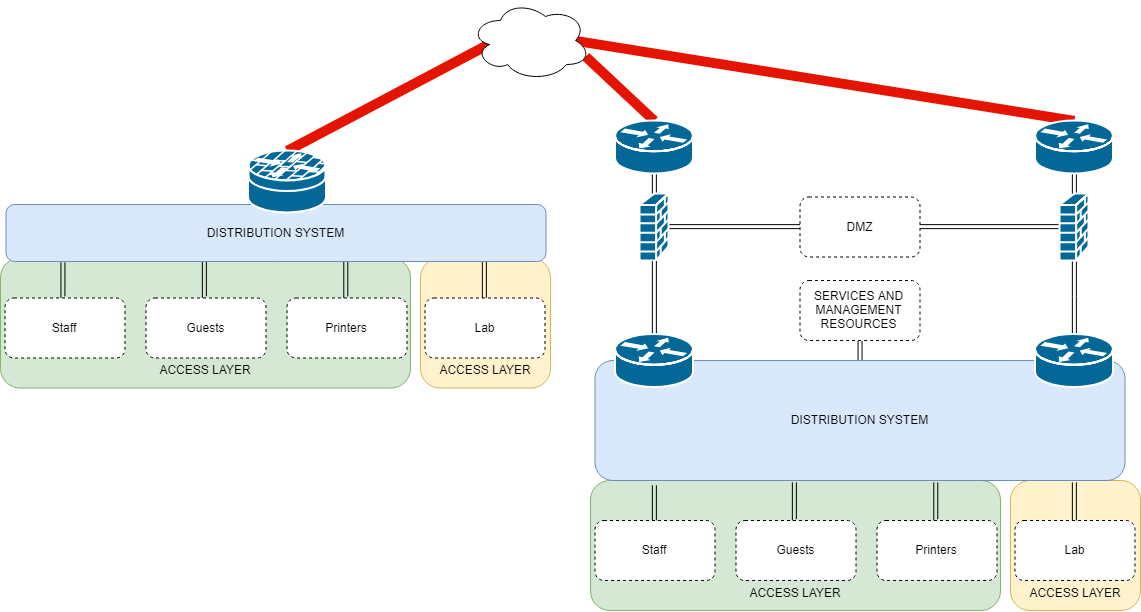
\includegraphics[width=\textwidth]{logicalview}
\label{logicalview}
\end{figure}

\subsubsection{Physical view}

We've used screenshots of our Packet Tracer implementation to produce the diagrams seen in Figure \ref{physicalviewhq} and \ref{physicalviewbranch}.

% TODO: update the physical diagrams

\begin{figure}[H]
\caption{Physical view of HQ (TEMPORARY)}
\centering
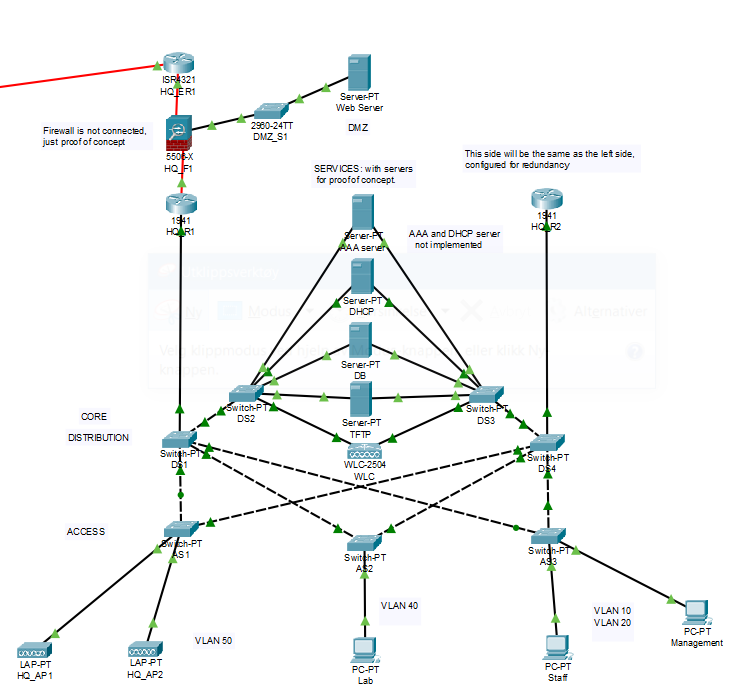
\includegraphics[width=\textwidth]{physicalviewhq}
\label{physicalviewhq}
\end{figure}

\begin{figure}[H]
\caption{Physical view of Branch (TEMPORARY)}
\centering
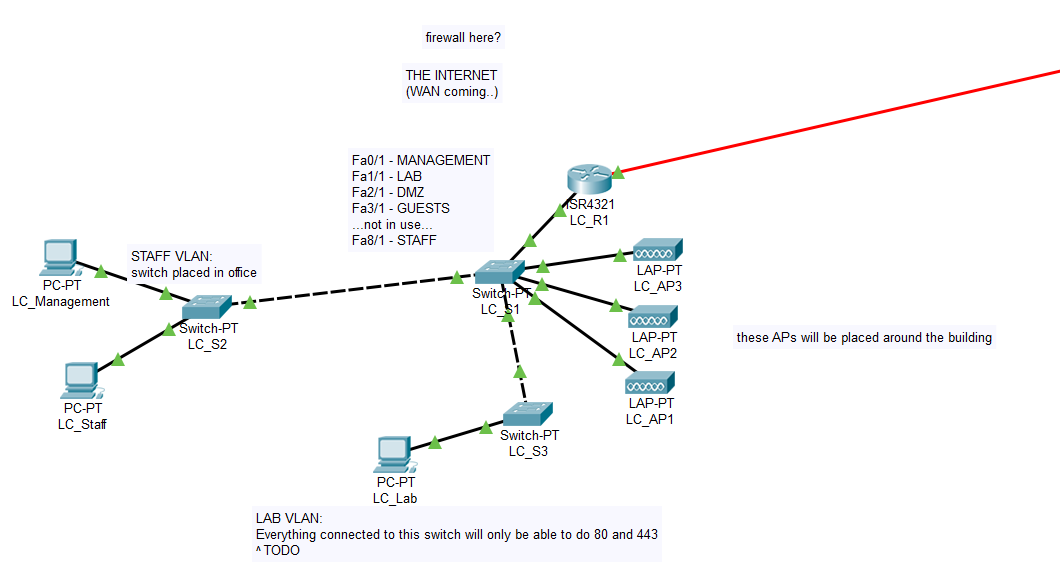
\includegraphics[width=\textwidth]{physicalviewbranch}
\label{physicalviewbranch}
\end{figure}


\subsection{WAN}

We use IPsec to create a site-to-site VPN tunnel from branches to the HQ. We chose VPN because it uses the public internet. Our traffic is encrypted, so security-wise this choice of technology should not restrict us. It does mean we have to settle for less performance though, but we're willing to accept this trade-off in favor of saving costs. 
\\
\\

%For the site to site WAN between HQ and branches, we have implemented an IPsec tunnel that traverses the internet, in order to connect branches and HQ without having to pay for a leased line, which is too expensive for us and therefore the reason to NOT use PPP or PPPoE, that cannot be transmitted over the internet as they are L2 protocols. IPsec on the other hand is a L3 protocol and therefore can be transmitted over the internet, which is a very affordable medium, also safe with IPsec encryption and we also don't really need the bandwidth of a leased line.

The WAN connection has two primary uses: To give Staff access to internal services located at the HQ, and to provide management access. In addition we also want to be able to VPN to HQ from an off-site location, so we need a VPN server with a pool of temporary IP addresses for remote commuters. This VPN connection would pass through an IPsec tunnel forwarded by the ISP to an off-site client.
\\
\\

%FIXME:--------isn't this more related to our demo configuration?
%The WAN connection is a series of serial cables from branches and HQ to each other, where there are own subnets between the edge routers. 
%The IPsec encrytion is configured between the edge routers only, and serves as an end to end encryption, to avoid MIM attacks, snooping and disclosure of sensitive information.

\subsection{VLANs and Subnets}

The goal when designing our VLAN's and subnets was simplicity. We chose to subnet our private addresses from the 10.0.0.0/8 private address range, as it gave us plenty of space to divide the subnets up how we wanted. We dedicate the second octet to indicate what location the subnet belongs to, where the value 1 indicates the HQ, and a value above 1 indicates a branch location. For example: 10.1.x.x is a subnet the HQ, and 10.2.x.x is a subnet at the first learning centre and so on.

This lets us create subnets that look very similar across locations, while letting a network engineer quickly see what location a particular IP address belongs to. We dedicate the third octet to indicate what VLAN the subnet belongs to, with the value of the octet being the same as the VLAN id. 10.1.10.x is a subnet for the management VLAN of the HQ, and 10.10.60.x is a subnet for the printer VLAN of location nr. 9. Combined with the fact that we reserve the first 10 hosts for static IPs in each subnet range, this leaves us with 244 available dynamic host addresses.

For the learning centres this is not a problem, as 244 guests are unlikely to be connected to the network at the same time. The HQ is more brittle, but we've concluded that 244 hosts should be enough there as well. Table \ref{VLANsubnettable} shows our VLAN's with their corresponding subnets. The character x refers to what location the subnet is on.

% TODO: 10.0.x.x = ipsec (subnet bruk mellom WAN linker)

% FIXME: H necessary?
% Forces table to show up under text
\begin{table}[H]
\caption{Table of VLANs with corresponding subnets}
\label{VLANsubnettable}
\begin{tabular}{|l|l|l|l|l|}
\hline
\textbf{VLAN Name} & \textbf{VLAN ID} & \textbf{Subnet} & \textbf{Excluded addresses} & \textbf{Available addresses} \\ \hline

Management     & 10      & 10.x.10.0/24 & 10.x.10.1 - 10.x.10.10 & 244 \\ \hline
Staff          & 20      & 10.x.20.0/24 & 10.x.20.1 - 10.x.20.10 & 244 \\ \hline
Services       & 30      & 10.x.30.0/24 & 10.x.30.1 - 10.x.30.10 & 244 \\ \hline
Lab            & 40      & 10.x.40.0/24 & 10.x.40.1 - 10.x.40.10 & 244 \\ \hline
Guest          & 50      & 10.x.50.0/24 & 10.x.50.1 - 10.x.50.10 & 244 \\ \hline
Printer        & 60      & 10.x.60.0/24 & 10.x.60.1 - 10.x.60.10 & 244 \\ \hline
DMZ            & 70      & 10.x.70.0/24 & 10.x.70.1 - 10.x.70.10 & 244 \\ \hline
Blackhole VLAN & 99      & N/A          & N/A                    & N/A \\ \hline
\end{tabular}
\end{table}

\subsection{Wireless}

% TODO: should use something other than PSK in the real setup?? google

We've chosen to build our wireless solution with Wireless Access Controllers (WLC's) and Lightweight Access Points (LWAP's). As we want as few resources as possible to be placed at the branch locations, the WLC's will be placed at the HQ. We will have redundancy in WLC by the use of the "High Availability" features that Cisco provides.~\cite{ciscoha}
\\
\\
This means that the LWAP's at the branches might encounter situations with no access to WLC's, but as this connection will benefit from the same redundancy as the one provided for services this will be relatively rare. We'd rather put resources into our one HQ than to spread resources around to each of the 17 branches.
\\
\\
The WLC's and LWAP's use CAPWAP to communicate, meaning all LWAP's are connected to access ports on the management VLAN. This unifies how we set up our IP addresses.
\\
\\
Our Wireless setup consists of two WLAN's, one for staff and one for guests. Both are configured with WPA2 level security. The staff WLAN is tagged to the staff VLAN, and the guest WLAN is mapped to the guest VLAN, this way staff and guest users connected over Wi-Fi will have the same rights as those connected physically.

\subsection{Lab}

%\notetous{Discuss how we implemented the lab environment}

The purpose of the labs was to provide an environment where visitors could experiment freely with information security concepts. This means that it is a security risk by design, so we have to be careful how we implement it. The labs will have their own physical switch, and the kinds of traffic that may pass through will be heavily restricted. Only browsing is allowed, so we restrict traffic to only established TCP for the protocols HTTP, HTTPS and DNS.
\\
\\
Some networking equipment will be placed in the lab to be used for experimentation, but we don't consider this a part of our network infrastructure.

% TODO: what traffic to allow? not just 80 443
% TODO: clean up plural vs singular
% TODO: elaborate

\subsection{Branch network discussion}

% TODO more sections?
%\notetous{Discuss topics specific to the branch network setup}

As seen in Figure \ref{physicalviewbranch}, the branch network is very simple. As all resources are located at the HQ, each branch only needs a router, a few switches and a few LWAP's to function. Each branch location will not have much traffic, so we can justify saving costs by placing the firewall, local DHCP server and the VPN termination at the router itself.

The LWAP's are configured through CAPWAP tunnels going to the WLC's at HQ. We could have set up redundant WLC functionality on each branch location, but decided against it because the cost of configuring this for each branch would be too high.
\\
\\
We don't consider the branch location as critical infrastructure. Rather than providing each branch location with redundancy, we place all resources at the HQ, and focus on providing redundancy there. This means that a branch might go down for a few days every once in a while. We consider this an accepted risk.

\subsection{HQ network discussion}

\subsubsection{Layout}

Initially we aimed for a three-tier architecture~\cite{threetier}, but found that a collapsed-core architecture~\cite{collapsedcore} suited our needs better. A collapsed-core architecture retains the redundacy of three-tier, but sacrifices some efficiency in favor of saving costs.
\\
\\
We have two routers and two switches set up to combine the core and distribution layer into a single layer. The services and management resources are given special treatment and placed in its own segment of the network, while the rest of the network is set up to use access switches with connections to both distribution/core layer switches to provide redundancy.
\\
\\
Physically each access layer switch is configured with access ports based on what users are found around the switch. Switches placed in the offices will have staff and management ports, while switches in lecture halls and such will have guest ports. LWAP's are connected to management switchports.

% TODO: elaborate?

\subsubsection{Redundancy}

As all of the branch locations rely on the HQ to operate, redundancy was an important topic to address. What really needs redundancy are the services and management resources. The fact that the rest of the HQ gets some redundancy is really just a bonus.

As shown in Figure~\ref{physicalviewhq}, the HQ has two links to the ISP through a duplicated setup of routers and switches. Important services and management resources are placed in the middle of the network, in between the two routers, as shown. They have dual Ethernet connections, one going to each ISP link. This way, if any of the equipment forming one of the paths to ISP goes down, the services and management resources will still have internet connectivity.
\\
\\
As we have have two gateways we need to use a "First Hop Redundancy" protocol to manage the default gateway. The options we looked at were HSRP, VRRP and GLBP. We went with GLBP because in addition to providing the redundancy we need, it also does load balancing, letting us utilize both of the gateway routers to their fullest. HSRP and VRRP would've provided redundancy, but not load balancing.


% TODO add note about use of HSRP in demo implementation?
% TODO refer to diagrams!!!!!!!!!! "as seen in \ref{...}" and so on

% not needed? talked about in above subsection
%\subsubsection{Services}
%\notetous{Discuss how services are handled at HQ}

\subsection{Methods for hardening}

\subsubsection{Physical information security} % FIXME: include "information" ?

% TODO 
% * staff kommer seg ikke inn i management. 
% * gjester er fysisk separaert fra staff. management kommer seg inn i management.


\textbf{Premise access}: The premises at HQ will be locked down. Access will be granted based on roles, and ID-card will be used to enforce this. Guests do not have access to the staff area, staff do not have access to the main server room, and so on. In addition the main server room will be secured with video surveillance and a mantrap. This way potential unauthorized access will be monitored, and failed attempt will result in the attacker being trapped.

\textbf{Device access}: Physical management ports will be secured with passwords, or turned off completely if they are not in use.

\subsubsection{Securing the LAN}
As layer 2 can be the weakest link in our network infrastructure we will implement different methods to prevent or mitigate potential attacks:

\textbf{Management and staff switch}: Whereas lab have a separate switch, management and staff share the same switch. Staff and management computers are connected physically and for new users to connect an admin must configure a new access port. For additional security all access ports on this switch use PVLAN edge to make it more difficult for a man-in-the middle attack against management traffic.

\textbf{STP manipulation attacks}: Our switches, especially in HQ, are set up for redundancy and use STP to prevent loops. All access port will have configured with PortFast and BPDU Guard to prevent an attacker becoming the root bridge.

\textbf{CAM table attack}: To prevent flooding of a switch's CAM table all access ports have port-security implemented. This also helps mitigate a DHCP starvation attack.

\textbf{VLAN hopping and double-tagging attack}: To prevent an attacker from spoofing a switch trunk all ports have disabled DTP (auto trunking). Ports available to users are explicitly assigned as access ports. To prevent a double-tagging attack trunks have a native Blackhole VLAN. Ports which are not in use are disabled. They are also configured as access ports to the Blackhole VLAN to force awareness of the configuration when turned back on.

\textbf{DHCP spoofing and DHCP starvation attacks}: To prevent rogue DHCP servers and further mitigate DHCP starvation we will use DHCP Snooping. It will be enabled for all user VLAN. While our upstream ports will be set to trusted, access port will have a limit to how many DHCP request it can send per second. However, we must take into account that it may take some time for the DHCP Snooping to finish the binding table. 

\textbf{ARP spoofing and ARP poisoning attacks}: In interaction with DHCP Snooping we will use DAI (Dynamic ARP Inspection) to prevent ARP spoofing and poisoning. Then the switch relays only valid ARP replies. Like DCHP snooping it will be enabled for user VLAN's and trusted ports will be on the same upstream interfaces. 

\textbf{IP and MAC spoofing attacks}: In addition we will implement IPSG (IP Source Guard) to prevent IP address and MAC address spoofing. It will be configured on untrusted access ports.

\subsubsection{Securing network infrastructure}

\textbf{Securing the router}: We use a defense-in-depth approach with a DMZ. Between our internal router and edge router we will have a firewall which will allow external networks to access our web server. On our edge router we will disable unnecessary services with the use of Cisco's auto secure function~\cite{autosecure}. All management access to router must be with the use of AAA and SSH if not connected to the console port. Remote access must have an established VPN connection beforehand.

\textbf{Firewalls}: The firewall is the networks first line of defence, and it it vitally important that we have a good firewall implementation. We will use next-gen firewalls~\cite{nextgenfirewall} in order to supply ourselves with both packet filtering and session analysis. With this we will always have a current threat picture due to the rapidly updating threat database of the firewall provider.

We have decided on firewalls from branch to HQ (Defence in Depth), and from the internet to endpoints on our network. This is to avoid split tunneling concerns. These concerns being that the users internet connection, if not filtered, may compromise the entire network; especially if the endpoint is a manager, as managers have clearance. We don't want to give a potential attacker this kind of access.

Our ACLs only allow staff-to-services and management-to-management traffic from branch to HQ.

\textbf{Authentication Authorization and Accounting}: Users within our network will have role-based access. We will implement this with the use of a TACACS+ server. The system admin of the site will also have a local user if connection to the server is lost. For every user in staff and management we will implement port based authentication (802.1x). This is to ensure that every action and access can be properly authorized as well as logged. The logging will be handled by a server and devices must share a NTP server for accuracy of events logged.

\textbf{ACLs}: In our infrastructure everyone should not be able to communicate with certain devices, or other users. The lab could be a potential security threat to the rest of our network. Therefore, we will implement ACLs that only allow the lab to only browse the internet, otherwise it should be a completely closed environment. Telnet will be explicitly disabled with the use of ACL. Only staff, services and management can communicate from branch to HQ and vice versa. Staff may only access the database to get documents required in their work.

\subsubsection{Endpoint security}

All endpoint devices must have software that prevents infection and spread of malware. This being due to the especially vulnerable nature of endpoints because of their interactions with a user.

Traditionally this is done firstly by installing some kind of anti malware software, in order to detect and mitigate malware threats. We could also provide the endpoint host with a host based IPS, to monitor and report on their system.
In accordance with this we can also install a host-based firewall to add to the security threats posed by incoming traffic, that may bypass the security measures of the network.

However, we did not decide to do this, as it simply is an outdated way of doing things on the scale we need it. Instead we opted for a more modern approach for endpoint security; by using:
Anti Malware Protection (AMP),
Email Security Appliances (ESA),
Web Security Appliances (WSA) 
and Network Admission Control (NAC). 
The combination of these different technologies and protocols gives us a good protection suite for the endpoint users and our whole network.

These technologies provide us with everything we need to efficiently secure the endpoints. Firstly AMP gives us an endpoint malware protection, secondly ESA provides us with email spam filtering even before the emails reach the endpoint.
WSA allows us to filter and blacklist websites that are malicious and or reputably unsafe. Last but not least we have NAC which permits only authorised and policy-compliant systems to connect to the network.

On the endpoint host we should use some form of data encryption in case of loss or theft. 

Now, we have all the tools we need to:
\begin{enumerate}
    \item Discover, enforce and protect before an event.
    \item Detect, block and defend during an event.
    \item Scope, contain and remediate after an event.
\end{enumerate}



\section{Our demo Packet Tracer implementation} \label{democonfigdiscussion}

% make sure to include that:
% * HSRP instead of GLBP
% * wireless not configured in packet tracer
% * list of what is implemented and what isn't?
% * explain how we simplified WAN for the demo

As part of the project we implemented part of our infrastructure in Packet Tracer. The configuration can be found in appendix \ref{config}. This section will provide some discussion around the demo implementation.

\subsection{WAN}

The WAN connection is a series of serial cables from branches and HQ to each other, where there are own subnets between the edge routers. 
The IPsec encrytion is configured between the edge routers only, and serves as an end to end encryption, to avoid MIM attacks, snooping and disclosure of sensitive information.

\subsection{HQ demo configuration}

Figure \ref{physicalviewhq} is taken from our PT implementation of the HQ. As you can see we have configured three access layer switches with a few machines attached to different access ports. The services and management resources area is set up with its own dedicated switches connected to the "distribution system", which is really just two switches connected to two gateway routers. The left gateway router shows the concept of how our defence-in-depth would be implemented, and also our IPSec connection to the branch location. The firewall is not plugged in, and the DMZ is not set up. In reality the firewall would be placed between the two routers, and traffic from the public web to our web server would be routed to the DMZ connected to the firewall, as illustrated by Figure \ref{logicalview}. The setup would be duplicated on the right gateway router.
\\
\\
In reality we would like to use GLBP for "first hop redundancy" and load balancing, but we did not figure out a way to do this in Packet Tracer. For demonstration purposes we configured HSRP on the routers instead.
\\
\\
The WLC would in reality be coupled with at least one standby controller, but we've only included one for the demo. It is plugged in, but does nothing. See \ref{demowireless} for further discussion on this topic.

% TODO: add lwaps to PT
% TODO: add refs to appendix configs

For hardening we have implemented port-security, mitigated STP manipulation, CAM table attacks, VLAN hopping and double-tagging attacks. However, we have not implemented DHCP Snooping, DAI or IPSG. Since our implementation is mainly in packet tracer these commands did have some limitations or were absent. DHCP Snooping would allegedly only work for VLAN1, for others it would display this error: "DHCP Snooping: The switch receives a DHCP DISCOVER message on an untrusted port. The device is not configured with a trusted port in the same vlan.  The device drops the packet.".

We have not implemented any of our services including the DHCP and AAA server. The DHCP pool for HQ and its VLANs are handled by the internal router. Secure management of devices like switches and routers in accordance with AAA is not implemented at all. In reality this is a big liability and would not be acceptable.

Our IPSec implementation defines ACLs that limit the communication from branch to HQ and vice versa. Branch management can access the tftp server. Branch staff can access the database for documents. Branch APs can communicate with the WLC. HQ management can talk to anyone in a branch for remote support and management.

\subsection{Branch demo configuration}

% TODO: write about address of AP's. Static cause of more security ACL?

As all the branches have similar configuration, we only implemented one in our demo. Figure \ref{physicalviewbranch} shows our implementation. % <- TODO: REWRITE
The router is very similar to how it would be configured in reality, the only different being that a firewall mechanism has not been set up. The LWAP's connected to the main switch are intended to be placed around the building, and would get their configuration from the WLC at HQ.

The hardening of branch is equal to our HQ implementation.

\subsection{Wireless demo configuration} \label{demowireless}

We had trouble with implementing WLC's and LWAP's properly in Packet Tracer, so we decided configure a physical WLC as a proof-of-concept of how the WLC at HQ in our demo would look like. The exported configuration is provided in appendix \ref{configwlc}. Two WLAN's Staff and Guest are set up with WPA2+PSK security. Note that the addresses used in the configuration file are wrong. All addresses starting with 192.168 should really start with 10.1. We configured it like this because we had trouble with the 10.0.0.0/8 range in the Cisco lab.

\section{Conclusion}

\notetous{An amazing conclusion that will knock the socks of Ernst boiiiiiiiiiiiiiiiiiii}

% BEGINNING OF REFERENCES

\clearpage % make references start on own page

% This makes LaTeX list all references in the bib file, instead of just 
% the ones that are cited with a \cite command
\nocite{*}

% BEGINNING OF APPENDIX

\bibliographystyle{acmdoi}
\bibliography{report}

\clearpage % make appendix start on own page
\appendix

\section{Our demo Packet Tracer implementation} \label{config}

\subsection{Branch} \label{configbranch}
\subsubsection{LC\_R1} \label{configwlc}
\inputminted[fontsize=\tiny,linenos,breaklines]{text}{./Config/Branch/LC-R1.txt}
\subsubsection{LC\_S1\_running-config} \label{configwlc}
\inputminted[fontsize=\tiny,linenos,breaklines]{text}{./Config/Branch/LC-S1-running-config.txt}
\subsubsection{LC\_S2\_running-config} \label{configwlc}
\inputminted[fontsize=\tiny,linenos,breaklines]{text}{./Config/Branch/LC-S2-running-config.txt}
\subsubsection{LC\_S3\_running-config} \label{configwlc}
\inputminted[fontsize=\tiny,linenos,breaklines]{text}{./Config/Branch/LC-S3-running-config.txt}

\subsection{HQ} \label{confighq}
\subsubsection{AccessSwitch-1} \label{configwlc}
\inputminted[fontsize=\tiny,linenos,breaklines]{text}{./Config/HQ/AccessSwitch-1.txt}
\subsubsection{AccessSwitch-2} \label{configwlc}
\inputminted[fontsize=\tiny,linenos,breaklines]{text}{./Config/HQ/AccessSwitch-2.txt}
\subsubsection{AccessSwitch-3} \label{configwlc}
\inputminted[fontsize=\tiny,linenos,breaklines]{text}{./Config/HQ/AccessSwitch-3.txt}
\subsubsection{DistributionSwitch-1} \label{configwlc}
\inputminted[fontsize=\tiny,linenos,breaklines]{text}{./Config/HQ/DistributionSwitch-1.txt}
\subsubsection{DistributionSwitch-2} \label{configwlc}
\inputminted[fontsize=\tiny,linenos,breaklines]{text}{./Config/HQ/DistributionSwitch-2.txt}
\subsubsection{DistributionSwitch-3} \label{configwlc}
\inputminted[fontsize=\tiny,linenos,breaklines]{text}{./Config/HQ/DistributionSwitch-3.txt}
\subsubsection{HQ\_ER1} \label{configwlc}
\inputminted[fontsize=\tiny,linenos,breaklines]{text}{./Config/HQ/HQ-ER1.txt}
\subsubsection{HQ\_R1} \label{configwlc}
\inputminted[fontsize=\tiny,linenos,breaklines]{text}{./Config/HQ/HQ-R1.txt}
\subsubsection{HQR2\_running-config} \label{configwlc}
\inputminted[fontsize=\tiny,linenos,breaklines]{text}{./Config/HQ/HQR2-running-config.txt}

\subsection{(Physical) WLC configuration} \label{configwlc}
\inputminted[fontsize=\tiny,linenos,breaklines]{text}{./wirelessimplementation/wlc.cisco}



\end{document}
